%%%%%%%%%%%%%%%%%%%%%%%%%%%%%%%%%%%%%%%%%%%%%%%%%%%%%%%%%%%%%%%%%%%%%%%%%%%%%%%%%%%%%%%%%%%%%%%%%%%%%%%
\chapter{Quantum Mechanics of Many-Body Systems}
\label{ch: Quantum Mechanics of Many-Body Systems}
%%%%%%%%%%%%%%%%%%%%%%%%%%%%%%%%%%%%%%%%%%%%%%%%%%%%%%%%%%%%%%%%%%%%%%%%%%%%%%%%%%%%%%%%%%%%%%%%%%%%%%%

One-particle quantum mechanics deals with systems consisting of only $\textit{one}$ particle. This is of course a natural and necessary starting point for all quantum mechanical considerations, where fundamental postualtes, formalism, quantization effects etc. can be introduced and discussed in piece and quiet without considering implications of real life systems. When this done, it is natural to move over to real physical systems which consists of more than one particle. These systems are often called many-body or many-particle systems in the litterature and provide a breeding ground for many-body theory and dusins of approximation schemes and methods. 

In this chapter, basic quantum mechanics of many-body systems are presented with an emphasize on the apparent everlasting many-body problem. 

%------------------------------------------------------------------------------------------------------
\section{The many-body problem}
\label{sec: the many-body problem}
%------------------------------------------------------------------------------------------------------
We consider an isolated system of $N$ identical particles that we assume can be treated non-relativistic. The properties of the system are given by the fundamental Schr�dinger equation,
\begin{align}
\label{eq:Many-body timedependent Schr�dinger equation}
i\hbar \frac{\partial}{\partial t}\ket{\Psi} = \OP{H}\ket{\Psi},
\end{align}
where $\ket{\Psi}$ is the $N$-particle wave function and $\OP{H}$ is the hamiltonian of the system defined as
\begin{align}
\label{exp:general hamilton operator}
\OP{H} = \OP{T} + \OP{V}.
\end{align}
The operators $\OP{T}$ and $\OP{V}$ denotes the kinetic energy and potential energy of the system, respectively. The time dependent Schr�dinger equation (\ref{eq:Many-body timedependent Schr�dinger equation}) provides all the properties of the system including the time evolution. It is appropriate to introduce the time elvolution operator $\OP{\mathcal{U}}$, which acting on a system state $\ket{\Psi(t_0)}$ yields the time evolution of the system at all times $t>t_0$,
\begin{align}
\label{exp:time evolution operator}
\ket{\Psi(t)} = \OP{\mathcal{U}}(t,t_0)\ket{\Psi(t_0)}.
\end{align}
Inserting (\ref{exp:time evolution operator}) into Eq.(\ref{eq:Many-body timedependent Schr�dinger equation}) yields the equation for the time-evolution operator,
\begin{align}
\label{eq:time evolution operator equation}
i\hbar\frac{\partial}{\partial t}\OP{\mathcal{U}}(t,t_0) = \OP{H}\OP{\mathcal{U}}(t,t_0).
\end{align}
When the hamiltonian is time independent, the time evolution operator reads
\begin{align}
\label{exp:time evolution operator 2}
\OP{\mathcal{U}}(t,t_0) = e^{-\frac{i}{\hbar}\OP{H}(t-t_0)}.
\end{align}
If we were to prepare a system in state $\ket{\Psi(t_0)}$ at time $t_0$, which for convenience often is chosen as $t_0=0$, the system state $\ket{\Psi(t)}$ for all $t>t_0$ is determined by simply letting the time evolution operator act on the initial state. It is already clear that the hamiltonian of the system determine the time evolution of the system, which in itself is a fundamental improtance, but it also provide the energy spectrum and eigenstates which are often our main interest. For example, an analytical expression of Eq. (\ref{exp:time evolution operator 2}) is only possible if the reference state is written as a linear combination of energy eigenstates. 

As pointed out before, the energy eigenvalues and eigenstates are of fundamental importance for every quantum mechanical considerations. When the hamiltonian of the system is stationary, the Schr�dringer equation (\ref{eq:Many-body timedependent Schr�dinger equation}) can be separated in time $t$ and coordinates of chosen representation (basis). This leads to the time-independent Schr�dinger (energy eigenvalue) equation
\begin{align}
\label{eq:Many-body timeindepundendent Schr�dinger equation}
\OP{H}\ket{\Psi_\lambda} = E_\lambda \ket{\Psi_\lambda},
\end{align}
where $\ket{\Psi_\lambda}$ is the energy eigenstate with corresponding eigenvalue $E_\lambda$ and $\lambda$ denote the set of quantum numbers needed for unique specification of the eigenstates. Up to now, no representation (basis) in the Hilbertroom has been chosen, and the previous discussion is valid for any favourite representation. We will in the following apply the coordinate representation, which is the most appropriate choice in the follwing treatment of the many-body problem. The Schr�dinger equation (\ref{eq:Many-body timeindependent Schr�dinger equation}) then reads
\begin{align}
\label{eq:Many-body timeindependent Schr�dinger equation coordinate representation}
\OP{H}(\vek{r}_1,\vek{r}_2,..,\vek{r}_N)\Psi_{\lambda}(\vek{r}_1,\vek{r}_2,..,\vek{r}_N) = E_\lambda \Psi_{\lambda}(\vek{r}_1,\vek{r}_2,..,\vek{r}_N),
\end{align}
where $\vek{r}_i$ are the spatial coordinates, with spin variables included, for the $i$'th particle. The hamiltonian is general, as pointed out before, the sum of the total kinetic energy and potential energy. The kinetic energy operator reads
\begin{align}
\label{exp:Kinetic energy operator}
\OP{T} &= \sum_{i=1}^N \OP{t}(\vek{r}_i) \\
       &= -\frac{\hbar^2}{2m}\sum_{i=1}^N \nabla_i^2.
\end{align}
In the general case, the potential energy operator is build up of $n$-body operators ($n = 1,2,..,N$), and is defined as an operator acting on $n$-particles. For example, the well-known coulomb interaction is a two-body interaction since it depends on the distance between two particles. The potential energy operator thus reads
\begin{align}
\label{exp:Potential energy operator}
 \OP{V} &= \OP{V}_1 + \OP{V}_2 + ... + \OP{V}_N\\
&= \sum_{i=1}^N \OP{v}_1(\vek{x}_i) + \sum_{i<j}^N \OP{v}_2(\vek{x}_i,\vek{x}_j) + ... + \sum_{i<j<..<l}^N \! \OP{v}_N(\vek{x}_i,\vek{x}_j,..,\vek{x}_l),
\end{align}
where the $\vek{x}_i$ is written instead of $\vek{r_i}$ to underline the fact that the potential in the general case also can be a function of for example momentum. In nuclear physics, it is normal to introduce two-body potential operators that is dependent on both spatial position and momentum. The fundamental strong interaction, which keep the nuclei tougether, also seems to exhibit three-body behaviour. This is fundamentally due to the fact that the interaction's exchange particles, called gluons, can couple to themselves. Relevant operators in real many-body systems involve not more than three-body operators, and is therefore usually omitted in the definition of the potential energy operator. For theoretical reasons, all $n$-body operators up are included in the general definition in (\ref{exp:Potential energy operator}).  

The eigenvalue equation in Eq. (\ref{eq:Many-body timeindependent Schr�dinger equation coordinate representation}), with the kinetic energy and potential energy operator defined in Eq. (\ref{exp:Kinetic energy operator}) and Eq.(\ref{exp:Potential energy operator}), respectively, is usually called the $\textit{quantum mechanical many-body}$ $\textit{problem}$. This is a highly non-trivial problem due to the interaction operators. In real-life systems, particles interact with each other, and one would at least have to include two-body operators in the potential energy. Even by only including the two-body interaction $\OP{v}_2$, the many-body problem cannot be solved exactly. In quantum mechanical treatment of many-body systems we are therefore forced to make use of different approxmation schemes and complex techniques. However, the natural starting point for all considerations of many-body systems is, despite the choice of method, the non-interacting system. 

%-------------------------------------------------------------------------------------------------------------------------------------------------------
\section{The non-interacting system}
\label{sec: the non-interacting system}
%-------------------------------------------------------------------------------------------------------------------------------------------------------
The general non-interacting (unperturbed) system consists of $N$ non-interacting particles subject to an external potential $u$. The hamiltonian reads
\begin{align}
\label{exp:Non-interacting hamiltonian}
\OP{H}_0 = \sum_{i=1}^N \OP{h}_0 = -\frac{\hbar^2}{2m}\sum_{i=1}^N \nabla_i^2 + \sum_{i=1}^N u(\vek{r}_i),
\end{align}
where the potential is assumed to be a function of spatial coordinates $\vek{r}_i$ including spin variable. The non-interacting Schr�dinger equation
\begin{align}
\label{eq:Non-interacting schr�dinger equation}
\OP{H}_0\Phi_a(\vek{r}_1,\vek{r}_2,..,\vek{r}_N) = E_a^0 \Phi_a(\vek{r}_1,\vek{r}_2,..,\vek{r}_N),
\end{align}
can be solved exactly by seperation of variables since the hamiltonian only consists of one-body operators. Inserting
\begin{align}
\label{exp:Non-interacting energy eigenvectors}
\Phi_a(\vek{r}_1,\vek{r}_2,..,\vek{r}_N) = \phi_\alpha(\vek{r}_1)\phi_\beta(\vek{r}_2)..\phi_\gamma(\vek{r}_N)
\end{align}
into Eq. (\ref{eq:Non-interacting schr�dinger equation}) yields $N$ identical single-particle equations, 
\begin{align}
\label{eq:Single-particle Schr�dinger equation}
\OP{h}_0 \phi(\vek{r}) = \epsilon \phi(\vek{r}).
\end{align}
We identify Eq. (\ref{eq:Single-particle Schr�dinger equation}) as the Schr�dinger equation for the system when only one particle is present. Solving this equation yields the set of single-particle energy eigenvalues $\kpr{\epsilon}$  and eigenfunctions $\kpr{\phi}$, and hence all the $N$-particle eigenfunctions in Eq. (\ref{exp:Non-interacting energy eigenvectors}) are determined. The total non-interacting energy eigenvalues are found by summing over all the single-particle energies,
\begin{align}
E_a^0 = \sum_{\alpha=1}^N \epsilon_{\alpha}.
\end{align}
A general state in the non-interacting system can be written as the linear combination of energy eigenstates,
\begin{align}
\Phi(\vek{r}_1,\vek{r}_2,..,\vek{r}_N) = \sum_{\kpr{\alpha\beta..\gamma}} c_{\alpha\beta..\gamma} \phi_\alpha(\vek{r}_1)\phi_\beta(\vek{r}_2)..\phi_\gamma(\vek{r}_N),
\end{align}
where $c_{\alpha\beta..\gamma}$ are the expansion coefficients satisfying the normalization condition
\begin{align}
\sum_{\kpr{\alpha\beta..\gamma}} \abs{c_{\alpha\beta..\gamma}}^2 = 1. 
\end{align}

The simple product form of the eigenfunctions in Eq. (\ref{exp:Non-interacting energy eigenvectors}) assumes that we can tell the particles apart. It would otherwise make no sense to claim that particle $1$ is in state $\phi_\alpha$, particle $2$ is in state $\phi_\beta$, and so on. In the classical regime, we can in principle always distinguish particles from each other, but in quantum mechanics, the situation is fundamentally different. When for example considering a system of electrons, we will never be able to tell them apart. Actually, it is not just that we do not happen to know; there is no such thing as ``this'' or ``that'' electron. Electrons are in fact $\textit{utually identical}$ in a way classical objects will never be. This is a feature which has to be baked into the wave function and which gives rise to two types of particles: fermions and bosons. 

%----------------------------------------------------------------------------------------------------------------------------------------------------------
\section{Identical particles}
\label{sec: identical particles}
%----------------------------------------------------------------------------------------------------------------------------------------------------------
The nature of identical particles gives rise to anti-symetric and symetric wave functions. A natural starting point is to investigate the permutation operator $\OP{P}$ and permutation symetri properties of the hamiltonian. The permutation operator $\OP{P}_{12}$ is defined by
\begin{align}
\label{exp:Permutation operator}
\OP{P}_{12} \phi_\alpha (\vek{r}_1)\phi_\beta (\vek{r}_2) = \phi_\alpha (\vek{r}_2) \phi_\beta (\vek{r}_1). 
\end{align}
In words, the permutation operator $\OP{P}_{ij}$ interchange the coordinates of particles $i$ and $j$. In quantum mechanics, the absolute squared of the wave function is interpreted as a probability density. Interchanging the coordinates of two completely identical particles should conserve this quantity, hence
\begin{align}
\abs{\Phi(..,\vek{r}_i,..,\vek{r}_j,..)}^2 = \abs{\Phi(..,\vek{r}_j,..,\vek{r}_i,..)}^2.
\end{align}
Mathematical this imply that 
\begin{align}
\Phi(..,\vek{r}_i,..,\vek{r}_j,..) = \pm \Phi(..,\vek{r}_j,..,\vek{r}_i,..),
\end{align}
which means that the total wave function is either symetric or anti-symetric with respect to the interchange of two particles. This is also shown by investigating the permutation operator and the hamiltonian. The hamiltonian for a system of identical particles is invariant under the interchange of particle coordinates. This imply that
\begin{align}
\fpr{\OP{H_0},\OP{P}_{ik}} = 0,
\end{align}
and hence we are in a position to construct eigenfunctions $\Phi_a$ of $\OP{H}_0$ that are also eigenfunctions of $\OP{P}_{ij}$ (see \cite{Dickhoff}). The eigenvalue equation of the permutation operator reads
\begin{align}
\OP{P}_{ij}\Phi_a(\vek{r}_1,..,\vek{r}_i,..,\vek{r}_j,..,\vek{r}_N) = \beta \Phi_a(\vek{r}_1,..,\vek{r}_j,..,\vek{r}_i,..,\vek{r}_N),
\end{align}
and the fact that 
\begin{align}
\label{exp:Permutation operator 2}
\OP{P}_{ij}^2 = 1,
\end{align}
implies that 
\begin{align}
\label{exp:Permutation operator 3}
\beta = \pm 1.
\end{align}
The pluss sign denotes systems of identical $\textit{bosons}$ where the wave function is symetric under the interchange of two particles. The minus sign denotes systems of $\textit{fermions}$ where the wave function is anti-symtetric under the interchange of two particles. Depending of whether the system consists of identical bosons or fermions, the eigenfunctions of Eq. (\ref{eq:Non-interacting schr�dinger equation}) must be either symetric or anti-symetric. Considering a two-particle system, the symetric and anti-symetric wave function reads
\begin{align}
\Phi_{+}(\vek{r}_1, \vek{r}_2) &= \frac{1}{\sqrt{2}}\fpr{\phi_\alpha(\vek{r}_1)\phi_\beta(\vek{r}_2) + \phi_\alpha(\vek{r}_2)\phi_\beta(\vek{r}_1)},\\
\Phi_{-}(\vek{r}_1, \vek{r}_2) &= \frac{1}{\sqrt{2}}\fpr{\phi_\alpha(\vek{r}_1)\phi_\beta(\vek{r}_2) - \phi_\alpha(\vek{r}_2)\phi_\beta(\vek{r}_1)}.
\end{align}
These states are eigenstates of the permutation operator $\OP{P}$ with eigenvalue $+1$ and $-1$, respectively. In addition they are also eigenstates of the non-interacting hamiltonian $\OP{H}_0$, both with energy eigenvalue
\begin{align}
E_0 = \epsilon_\alpha + \epsilon_\beta.
\end{align}
In the general case, a symetric and anti-symetric wave function for the $N$-patricle system can be generated by a symetrizer and antisymetrizer operator, respectively, by acting on the product state in Eq. (\ref{exp:Non-interacting energy eigenvectors}). The symetrizer is defined as
\begin{align}
\label{exp:Antisymmetrizer operator}
\OP{\mathcal{A}} = \frac{1}{\sqrt{N!}}\sum_p (-1)^p \OP{P}_p,
\end{align}
and the antisymetrizer as
\begin{align}
\label{exp:Symmetrizer operator}
\OP{\mathcal{S}} = \frac{1}{\sqrt{N!}}\sum_p \OP{P}_p.
\end{align}
A symetric and antisymetric $N$-particle wave function is then generated by letting these operators act on the product states,
\begin{align}
\label{exp:Symmetrized energy eigenfunctions}
\Phi_S(\vek{r}_1,\vek{r}_2,..,\vek{r}_N) &=  \frac{1}{\sqrt{n_\alpha!n_\beta!..n_\gamma!}}\OP{\mathcal{S}} \phi_\alpha(\vek{r}_1) \phi_\beta(\vek{r}_2)..\phi_\gamma(\vek{r}_N)\\
\label{exp:Antisymetrized energy eigenfunctions}
\Phi_{AS}(\vek{r}_1,\vek{r}_2,..,\vek{r}_N) &= \OP{\mathcal{A}} \phi_\alpha(\vek{r}_1) \phi_\beta(\vek{r}_2)..\phi_\gamma(\vek{r}_N).
\end{align}
An important feature of the fermionic antisymetric wave function is that every single-particle state $\phi_\alpha$ can only be occupied by $\textit{one}$ electron only. If we were to put two fermions in the same single-particle state, the wave function would simply be equal to zero, which is completely nonsense. This is the famous Pauli exclusion principle. The bosonic symetric wave function, on the other hand, has no occupancy limit within each single-particle wave function. Bosons and fermions manifest themselves in the nature as $\textit{integer}$ and $\textit{half integer}$ spin particles, respectively. In relativistic quantum mechanics, this feature can actually be proved. We refer to standard textbooks in relativistic quantum field theory.

In general, a system of bosons and a system of fermions manifest quite different properties due to the symetric and antisymetric wave functions. For example, identical bosons tend to be somewhat closer together, and identical fermions somewhat farther apart, than distinguishable particles in the same single-particle states. This can be shown explicit by calculating the two-particle system expectation value $\forv{(x_1 - x_2)^2}$ (coordinates $1$-dimension). After some tedious algebra (see \cite{Griffiths}), the bosonic/fermionic expectation value reads
\begin{align}
\forv{(x_1-x_2)^2}_\pm = \forv{(x_1-x_2)^2} \mp 2\abs{\forv{x}_{\alpha\beta}}^2, 
\end{align}
where $\forv{(x_1-x_2)^2}$ denote the expectation (reference) value for distinguishable particles, and
\begin{align}
\forv{x}_{\alpha \beta} = \int \! x \phi_\alpha^\ast(x)\phi_\beta(x)dx.
\end{align}
When the single-particle wave functions overlap, the system behaves as though there were an attraction force between identical bosons, and a repulsion force between identical fermions. In the literature, this is called the exchange force. It is important to note that this is not a real force, but merely a geometrical consequence of the wave function symetrization.

We have till now omitted the spin in our discussion. The $\textit{total}$ non-interacting energy eigenfunctions consist of a spatial part and a spin part, connected together with a tensor product,
\begin{align}
\Phi_{TOT} = \Phi \otimes \chi.
\end{align}
It is the $\textit{total}$ wave function that should obey the symetrization requirements, not just the spatial part. A system of fermions require the spatial part and the spin part to have opposite symetrization, while a system of bosons require equal symetrization. All expressions till now are still valid by including the spin inside the total single-particle quantum number $\alpha$.

As pointed out before, the basic fundament for all quantum mechanical treatment of interacting many-body systems is the non-interacting system, which is the natural first approximation. Important features of the full wave function and the hamiltonian can be extracted, giving essential and fundamental information of system from the very start, both in the sense of physical reality and numerical expenditure. In the next section, the treatment of many-body systems with interacting particles is presented. 

%----------------------------------------------------------------------------------------------------------------------------------------------------------
\section{The interacting many-body system}
\label{sec: the interacting many-body system}
%----------------------------------------------------------------------------------------------------------------------------------------------------------
In this section, the interacting many-body system is considered. We will limit the discussion to fermionic systems with antisymetric wave function. The Schr�dinger equation reads
\begin{align}
\OP{H}\Psi_\lambda(\vek{r}_1,\vek{r}_2,..,\vek{r}_N) = E_\lambda\Psi_\lambda(\vek{r}_1,\vek{r}_2,..,\vek{r}_N).
\end{align}
As pointed out before, this equation cannot, in general, be solved exactly for $N>1$. Nevertheless, general properties of the wave function $\Psi_\lambda$ can be determined by looking at the symmetry of the hamiltonian $\OP{H}$. For example, letting $\OP{H}$ be rotational invariant, i.e. 
\begin{align}
\fpr{\OP{H},\OP{R}} = 0,
\end{align}
where $\OP{R}$ is the intrinsic spin rotation operator, the total spin of the system is said to be conserved. This means that acting with $\OP{H}$ on $\textit{any}$ $N$-particle wave function $\ket{f} \in \mathcal{H}_N$ with spin $s_f$,
\begin{align}
\OP{H}\ket{f} = \ket{g},
\end{align}
yield a $N$-particle function $\ket{g} \in \mathcal{H}_N$ with the same spin. This allow us to diagonalize the hamiltonian seperate for each total spin, so that we obtain reduction of the matrix dimensionality.  
\begin{tikzpicture}
\draw (0,0) -- (2,0);
\draw (2,0) -- (2,2);
\draw (2,2) -- (0,2);
\draw (0,2) -- (0,0);
\draw (3,0) -- (5,0);
\draw (5,0) -- (5,2);
\draw (5,2) -- (3,2);
\draw (3,2) -- (3,0);
%(1,1) circle (2pt)
%(2,1) circle (2pt)
%(2,0) circle (2pt);
%\draw (0,0) .. controls (1,1) and (2,1) .. (2,0);
\end{tikzpicture}

An other important symmetry property of the hamiltonian is the permutation symmetry. In the previous section, the permutation operator was defined in Eq. (\ref{exp:Permutation operator}). The full interacting hamiltonian for a system of identical particles are invariant under the permutation of particle coordinates, i.e.
\begin{align}
\fpr{\OP{H},\OP{P}} = 0. 
\end{align}
Hence we can construct a set of functions $\kpr{\Psi}$ that are eigenfunctions of both $\OP{H}$ and $\OP{P}$. The eigenvalue equation for the permutation operator reads
\begin{align}
\OP{P}_{ij}\Psi_\lambda(\vek{r}_1,..,\vek{r}_i,..,\vek{r}_j,..,\vek{r}_N) = \beta \Psi_\lambda(\vek{r}_1,..,\vek{r}_i,..,\vek{r}_j,..,\vek{r}_N).
\end{align}
Since Eq. (\ref{exp:Permutation operator 2}) and Eq. (\ref{exp:Permutation operator 3}) still holds, the total wave function $\Psi_\lambda$ is either symetric or antisymetric depending on whether the system consits of bosons or fermions. 

%----------------------------------------------------------
\subsection{Hilbert spaces of distinguishable particles}
\label{subsec: hilbert spaces of distinguishable particles}
%----------------------------------------------------------
Consider a system of $N$ distinguishable particles. The $\textit{total wave function}$ lives in the infinite $N$-particle Hilbert space $\mathcal{H}_N$. Assume we have found a one-particle infinite basis set $\mathcal{B}_1^\alpha = \kpr{\ket{\alpha}}$ which span the $1$-particle hilbertspace $\mathcal{H}_1$. The quantum number $\alpha$ can correspond to position, momentum or your favourite basis functions that fullfill the orthonormality relation and completeness relation. The $N$-particle Hilbert space can be constructed by building it out of $N$ one-particle spaces,
\begin{align}
\mathcal{H}_N = \mathcal{H}_{1_1 \otimes 1_2 \otimes ... \otimes 1_N} = \mathcal{H}_{1_1} \otimes \mathcal{H}_{1_2} \otimes ... \otimes \mathcal{H}_{1_N},  
\end{align}
which is called the $\textit{direct product space}$. $\OP{H}_{1_i}$ denote the $1$-particle Hilbert space for particle $i$. The basis set of the $N$-particle product space can be constructed in a similar fashion,
\begin{align}
\label{exp:Direct product states}
\ket{\alpha \beta .. \gamma} = \ket{\alpha} \otimes \ket{\beta} \otimes .. \otimes \ket{\gamma},
\end{align}
which is often refered to as the $\textit{direct product basis}$. See \cite{Shankar} for a complete discussion. When considering a system of $N$ distinguishable particles, the total wave function can be written as a linear combination of the product states,
\begin{align}
\ket{\Psi_D} = \sum_{\kpr{\alpha\beta..\gamma}} c_{\alpha\beta..\gamma}\ket{\alpha\beta..\gamma}.
\end{align}
In the coordinate representation, the wave function then reads
\begin{align}
\label{exp:Distinguishable particles 1}
\Psi_D(\vek{r}_1,\vek{r}_2,..,\vek{r}_N) =  \sum_{\kpr{\alpha\beta..\gamma}} c_{\alpha\beta..\gamma}\phi_\alpha(\vek{r}_1)\phi_\beta(\vek{r}_2)..\phi_\gamma(\vek{r}_N).
\end{align}
In Eq. (\ref{exp:Distinguishable particles 1}), the single-particle basis functions are written as $\phi$ (see section \ref{sec: The non-interacting system}) to underline the fact that the $\textit{natural}$ and $\textit{good}$ basis functions are in most cases those generated from the non-interacting system. Nevertheless, Eq. (\ref{exp:Distinguishable particles 1}) are valid for $\textit{any}$ single-particle basis set.

%---------------------------------------------------
\subsection{Bosonic and fermionic Hilbert spaces}
\label{subsec: bosonic and fermionic hilbert spaces}
%---------------------------------------------------
Consider a system of $N$ bosonic or fermionic particles. As pointed out before, the total $N$-particle wave function must satisfy symetrization requirements. We denote the $N$-particle Hilbert space of symmetric bosonic vectors $\mathcal{H}^S_N$ and the Hilbert space of antisymmetric fermionic vectors $\mathcal{H}^{A}_N$. In the two-particle system, to each pair of product states $\ket{\alpha\beta}$ and $\ket{\beta \alpha}$, there exist one symmetric bosonic vector and one antisymmetric fermionic vector. When $\alpha = \beta$, the product state is already symmetric, and a fermionic state does not exist due to Pauli exclusion principle. The two-particle Hilbert space has thus enough basis states to form one symmetric space and one antisymmetric space, written as
\begin{align}
\mathcal{H}_2 = \mathcal{H}^S_2 \oplus \mathcal{H}^A_2,
\end{align}
and in the general $N$-particle case,
\begin{align}
\mathcal{H}_N = \mathcal{H}^S_N \oplus \mathcal{H}^A_N.
\end{align}
In the literature, one often view $\mathcal{H}^S_N$ and $\mathcal{H}^A_N$ as subspaces of $\mathcal{H}_N$. Given a system of $N$ bosons or fermions, the state will be an element of $\mathcal{H}_N^S$ or $\mathcal{H}_N^A$, respectively. It can also be shown that a system that initially starts out in the symmetric or antisymmetrix subspace, will remain in the same subspace for all later times. Hence, by considering a system of bosons (fermions) it is sufficient to only deal with the symmetric (antisymmetric) subspace.

The basis functions for the symmetric $N$-particle Hilbert space and the antisymmetric $N$-particle Hilbert space can be constructed from an orthonormal and colomplete single-particle basis set. As was the case for distinguishable particles, the direct product states in Eq. (\ref{exp:Direct product states}) do not constitute a basis for the symmetric and antisymmetric subspaces. As can be done for all wave functions, the bosonic and fermionic states can be written as a linear combination of a (at the moment unknown) basis set,
\begin{align}
\ket{\Psi_B} &= \sum_i c_i \ket{i}\\
\ket{\Psi_F} &= \sum_j c_j \ket{j}.
\end{align}
To have $\ket{\Psi_S}$ and $\ket{\Psi_A}$ symmetric and antisymmetric, respectively, require the basis functions $\ket{i}$ to be symmetric and $\ket{j}$ to be antisymmetric. Since the product states are not all symmetric and antisymmetric, they cannot be used as basis functions. In section \ref{sec: Identical particles}, symmetric and antisymmetric states were constructed from the product states, see Eq. (\ref{exp:Symmetrized energy eigenfunctions}) and Eq. (\ref{exp:Antisymetrized energy eigenfunctions}). $\textit{These}$ functions have the correct symmetry in addition to inherit the orthonormality from the product states. Hence, 
\begin{align}
\ket{i} &=  \frac{1}{\sqrt{n_\alpha!n_\beta!..n_\gamma!}}\OP{\mathcal{S}} \ket{\alpha\beta..\gamma}\\
\ket{j} &= \OP{\mathcal{A}} \phi_\alpha(\vek{r}_1) \ket{\alpha\beta..\gamma},
\end{align}
where the symmetrizer operators are defined in Eq. (\ref{exp:Symmetrizer operator}) and Eq. (\ref{exp:Antisymmetrizer operator}). $\textit{Any}$ orthonormal and complete single-particle basis can be used. Nevertheless, as was the case for distinguishable particles, the $\textit{good}$ single-particle basis is often the non-interacting set. Written in the coordinate representation, the bosonic and fermionic wave function reads
\begin{align}
\Psi_B(\vek{r}_1,\vek{r}_2,..,\vek{r}_N) &=  \sum_{\kpr{\alpha\beta..\gamma}} \frac{c_{\alpha\beta..\gamma}}{\sqrt{n_\alpha!n_\beta!..n_\gamma!}}\OP{\mathcal{S}} \phi_\alpha(\vek{r}_1) \phi_\beta(\vek{r}_2)..\phi_\gamma(\vek{r}_N)\\
\label{exp:Fermionic wave function}
\Psi_{F}(\vek{r}_1,\vek{r}_2,..,\vek{r}_N) &= \sum_{\kpr{\alpha\beta..\gamma}} d_{\alpha\beta..\gamma}\OP{\mathcal{A}} \phi_\alpha(\vek{r}_1) \phi_\beta(\vek{r}_2)..\phi_\gamma(\vek{r}_N).
\end{align}
The fermionic basis functions in Eq. (\ref{exp:Fermionic wave function}) can be written as a determinant, called $\textit{Slater determinant}$,
\begin{align}
\label{exp: Slater determinant}
\Phi_{\alpha\beta..\gamma}(\vek{r}_1,\vek{r}_2,..,\vek{r}_N) = \frac{1}{\sqrt{N!}}\left|\begin{array}{cccc}\phi_\alpha(\vek{r}_1) & \phi_\beta(\vek{r}_1) & \cdots & \phi_\gamma(\vek{r}_1)\\
\phi_\alpha(\vek{r}_2) & \phi_\beta(\vek{r}_2) & \cdots & \phi_\gamma(\vek{r}_2) \\ \vdots & \vdots & \vdots & \vdots\\ 
\phi_\alpha(\vek{r}_N) & \phi_\beta(\vek{r}_N) & \cdots & \phi_\gamma(\vek{r}_N)\end{array} \right|,
\end{align}
where $\Phi$ and $\phi$ are used to indicate that we are working with the good basis, i.e. the non-interacting set. But as pointed out before, every set of single-particle functions satisfying basis requirements, can be used. A general fermionic wave function can thus be expanded as an infinite series of Slater determinants,
\begin{align}
\Psi_{F}(\vek{r}_1,\vek{r}_2,..,\vek{r}_N) &= \sum_{\kpr{\alpha\beta..\gamma}} d_{\alpha\beta..\gamma} \Phi_{\alpha\beta..\gamma}(\vek{r}_1,\vek{r}_2,..,\vek{r}_N).
\end{align}

%-------------------------------------------------------------------------------------------------------------------------------------------------------
\section{Correlations in many-body systems}
\label{sec: correlations in many-body systems}
%-------------------------------------------------------------------------------------------------------------------------------------------------------

%-------------------------------
\section{Second Quantization}
\label{sec: Second Quantization}
%-------------------------------
In the previous section, the so-called slater determinant was introduced. Eq. (\ref{exp: Slater determinant}) clearly shows by construction that one may never assign one-to-one correspondence between single-particle states and particle coordinates, which is a direct consequence of the particles identical nature. The only thing we can say is what single-particle orbital is occupied. Thus the full slater determinant in Eq. (\ref{exp: Slater determinant}) include much redundant information, and it is therefore appropriate to characterize slater determinants by single-particle states only. Hence we write the slater determinant in Eq. (\ref{exp: Slater determinant}) in the more abstract, yet simpler, form
\begin{align}
\Phi_{\alpha_1\alpha_2..\alpha_N} \equiv \ket{\alpha_1\alpha_2..\alpha_N}.
\end{align}
This notation is called the occupancy representation, for the obvious reason. This form of the antisymmetrized wave function does not explicit reflect the antisymmetry in the particle coordinates. Nevertheless, the slater determinant changes sign in permutation of two columns, so that the abstract notation also is antisymmetric to permutation of single-particle orbitals,
\begin{align}
\label{exp: Slater determinant antisymmetry}
\ket{\alpha_1..\alpha_i..\alpha_j..\alpha_N} = -\ket{\alpha_1..\alpha_i..\alpha_j..\alpha_N}.
\end{align}
The full potential of the occupancy notation for antisymmetrized states is released when creation and annihilation operators is introduced. Creation operators create fermions in single-particle states, while the annihilation operators remove fermions from single-particle states. In many-body theory literature, this formalism is called second quantization, even though it has not the direct physical interpretation as in relativistic quantum field theory, where the second quantization originally was introduced. In the field theory, this formalism reflects physical processes such as creation and annihilation of quanta. In the non-relativistic quantum field theory, the formalism of creation and annihilation operators is intruduced for appropriate reasons. For example, the second quantization formalism allow us to use the pratical particle-hole formalism. 

%--------------------------------------------------
\subsection{Creation and annihilation operators}
\label{subsec: Creation and annihilation operators}
%--------------------------------------------------
The creation and annihilation operators are defined as operators that create and annihilate particles in single-particle states. We define the fermionic creation operator $\cre{\alpha}$ as
\begin{align}
\label{exp: Creation operator 1}
\cre{\alpha}\ket{0} &\equiv \ket{\alpha}\\
\label{exp: Creation operator 2}
\cre{\alpha}\ket{\alpha_1\alpha_2..\alpha_N} &\equiv \ket{\alpha\alpha_1\alpha_2..\alpha_N}\\
\label{exp: Creation operator 3}
\cre{\alpha}\ket{\alpha_1\alpha_2..\alpha..\alpha_N} &\equiv 0.
\end{align}
In Eq. (\ref{exp: Creation operator 1}), the creation operator acts on the vacuum state, that is the state with no particles, and creates a fermion in state $\alpha$. In Eq. (\ref{exp: Creation operator 2}), the operator acts on the $N$-fermion state with single-particle states $\alpha_i \neq \alpha$, yielding a $N+1$-fermion system where a fermion in state $\alpha$ has been created. When the creation operator acts on the $N$-fermion state in Eq. (\ref{exp: Creation operator 3}) where the single-particle orbital $\alpha$ already is occupied, the result is zero. The definitions above imply that the full slater determinant can be written as a product of creation operators,
\begin{align}
\label{exp: Slater determinant second quantization}
\ket{\alpha_1\alpha_2..\alpha_N} = \cre{\alpha_1}\cre{\alpha_2}..\cre{\alpha_N}\ket{0}.
\end{align}
Combining Eq. (\ref{exp: Slater determinant second quantization}) and Eq. (\ref{exp: Slater determinant antisymmetry}) into 
\begin{align}
\cre{\alpha_1}..\cre{\alpha_i}..\cre{\alpha_j}..\cre{\alpha_N}\ket{0} = -\cre{\alpha_1}..\cre{\alpha_j}..\cre{\alpha_i}..\cre{\alpha_N}\ket{0},
\end{align}
yields the commutation relation
\begin{align}
\label{exp: Creation operator commutation relation}
\kpr{\cre{\alpha},\cre{\beta}} = \cre{\alpha}\cre{\beta} + \cre{\beta}\cre{\alpha} = 0. 
\end{align}
By taking the hermitian conjugate of the creation operator we obtain the operator $\an{{\alpha}} = \pr{\cre{\alpha}}^\dagger$. First of all, the hermitian conjugate of Eq. (\ref{exp: Creation operator commutation relation}) yield the commutation relation
\begin{align}
\label{exp: Annihilation operator commutation relation}
\kpr{\an{{\alpha}},\an{{\beta}}} = \an{{\alpha}}\an{{\beta}} + \an{{\beta}}\an{{\alpha}} = 0. 
\end{align}
The action of $\an{\alpha}$ on a slater determinant reads,
\begin{align}
\label{exp: Annihilation operator 1}
\an{\alpha}\ket{0} &= 0\\
\label{exp: Annihilation operator 2}
\an{\alpha_i}\ket{\alpha_1..\alpha_{i-1}\alpha_i\alpha_{i+1}..\alpha_N} &= (-1)^p\ket{\alpha_i\alpha_1..\alpha_{i-1}\alpha_{i+1}..\alpha_N} = (-1)^p \ket{\alpha_1..\alpha_{i-1}\alpha_{i+1}..\alpha_N}\\
\label{exp: Annihilation operator 3}
\an{\alpha}\ket{\alpha_1\alpha_2..\alpha_N} &= 0.
\end{align}
These realtions follow from the definition of the creation operator in Eq. (\ref{exp: Creation operator 1}), (\ref{exp: Creation operator 2}) and (\ref{exp: Creation operator 3}). We refer to \cite{Dickhoff} for a further discussion. In Eq. (\ref{exp: Annihilation operator 1}), the annihilation operator acts on the vacuum state, yielding zero. In Eq. (\ref{exp: Annihilation operator 2}), the annihilation operator removes a fermion from single-particle state $\alpha_i$. When the $N$-particle state does not include the removal state, which is the case in Eq. (\ref{exp: Annihilation operator 3}), the result is zero. These results clarify why $\an{\alpha}$ is called the fermionic annihilation (destruction) operator. The commutation relation between the creation and annihilation operator (see \cite{Dickhoff}) reads
\begin{align}
\label{exp: Creation and annihilation commutation relation}
\kpr{\cre{\alpha},\an{\beta}} = \delta_{\alpha\beta}.
\end{align}

Since all antisymmetric wave functions are superpositions of slater determinants, we are noe in a position to express these states as products of creation operators acting on the vacuum state. The particle-hole formalism allow us to introduce a new reference state, which can be used to shrink the dimesionality of the problem. Before we discuss this formalism, operators in second quantization is introduced. 

%-----------------------------------------------
\subsection{Operators in second quantization}
\label{subsec: Operators in second quantization}
%-----------------------------------------------
We are now in a position to express many-fermion states by creation and annihilation operators. In many-body theory, however, it almost always comes down to evaluating matrix elements or expectation values of operators. Thus to get full profit of the second quantization formalism we also have to express operators by creation and annihilation operators. Operators expressed in the formalism of second quantization also have the convenient property that they do not depend on the numbers of particles in the system. They work in the so-called Fock space (see \cite{Dickhoff}), which is the vector space constructed by the direct sum of the vacuum space, the single-particle Hilbert space, the two-particle Hilbert space, and so forth, yielding
\begin{align}
\mathcal{F} = \bigoplus_{n=0}^\infty \mathcal{H}^{A}_n. 
\end{align}
This gives us a huge advantage in the way that we for example can work with a given ab initio method, deduce equations, and so forth, without specifying the size of the system. We will in the following only consider the second quantized form of one- en two-body operators. The formalism may be applied to higher order operators, and we refer the reader to any textbook on many-body theory. 

A one-body operator $\OP{F}$ consists of a sum of single-particle operators $\OP{f}$. In an $N$-particle space, the operator reads
\begin{align}
\OP{F} = \sum_{i=1}^N \OP{f}(i),
\end{align}
where $f(i)$ acts on particle $i$ and $N$ is the total number of particles. Given an arbitrary single-particle basis $\kpr{\ket{\alpha}}$, the second quantized formulation of a generic one-body operator $\OP{F}$ (see deduction in \cite{Dickhoff}) reads
\begin{align}
\OP{F} = \sum_{\alpha\beta}\for{\alpha}{f}{\beta}\cre{\alpha}\an{\beta}.
\end{align}
The operator $\OP{F}$ thus annihilates a particle in state $\beta$ and creates a particle in state $\alpha$ with probability amplitude $\for{\alpha}{f}{\beta}$. 

A two-body operator $\OP{V}$ in the $N$-particle space is given by
\begin{align}
\OP{V}_N = \sum_{i<j}^N \OP{v}(i,j),
\end{align}
where $\OP{v}(i,j)$ acts on particle $i$ and $j$, and $N$ is the number of particles in the system. Given an arbitrary two-particle basis product basis $\kpr{\ket{\alpha\beta}}$, the second quantized formulation of a generic two-body operator $\OP{V}$ (see deduction i \cite{Dickhoff}) reads
\begin{align}
\label{exp: Two-body operator second quantization}
\OP{V} &= \frac{1}{2}\sum_{\alpha\beta\gamma\delta}\for{\alpha\beta}{v}{\gamma\delta}\cre{\alpha}\cre{\beta}\an{\delta}\an{\gamma}\\
&= \frac{1}{4}\sum_{\alpha\beta\gamma\delta}\for{\alpha\beta}{v}{\gamma\delta}_{AS}\cre{\alpha}\cre{\beta}\an{\delta}\an{\gamma},
\end{align}
where the antisymmetrized matrix element is defined as
\begin{align}
\for{\alpha\beta}{v}{\gamma\delta}_{AS} = \for{\alpha\beta}{v}{\gamma\delta} - \for{\alpha\beta}{v}{\delta\gamma}.
\end{align}
The operator $\OP{V}$ annihilates a particle from state $\gamma$ and $\delta$, and creates a particle in state $\alpha$ and $\gamma$, with probability amplitude $\frac{1}{4}\for{\alpha\beta}{v}{\gamma\delta}_{AS}$.

We have now established the formalism of second quantization for both antisymmetric wave functions, and one- and two-body operators. As pointed out before, in quantum mechanical many-body calculations, we often end up with evaluating matrix elements. As an example, consider 
\begin{align}
\for{\alpha_1\alpha_2}{\OP{V}}{\alpha_3\alpha_4},
\end{align}
where $\ket{\alpha_1\alpha_2}$ and $\ket{\alpha_3\alpha_4}$ denote slater determinants. We now incorporate the formalism of second quantuzation, with 
\begin{align}
\bra{\alpha_1\alpha_2} &= \bra{0}\an{\alpha_1}\an{\alpha_2}\\
\ket{\alpha_3\alpha_4} &= \cre{\alpha_3}\cre{\alpha_4}\ket{0},
\end{align}
and $\OP{V}$ given by Eq. (\ref{exp: Two-body operator second quantization}). This yields
\begin{align}
\for{\alpha_1\alpha_2}{\OP{V}}{\alpha_3\alpha_4} = \frac{1}{4}\sum_{\alpha\beta\gamma\delta}\for{\alpha\beta}{v}{\gamma\delta}_{AS}\for{0}{\an{\alpha_1}\an{\alpha_2}\cre{\alpha}\cre{\beta}\an{\delta}\an{\gamma}\cre{\alpha_3}\cre{\alpha_4}}{0}. 
\end{align}
Hence we are ending up with evaluating vacuum expectation values of products of creation and annihilation operators. These expressions can be evaluated by using the anticommutation relations in Eq. (\ref{exp: Creation operator commutation relation}), (\ref{exp: Annihilation operator commutation relation}) and (\ref{exp: Creation and annihilation commutation relation}). However, this approach can be quite tedious even for relatively short operator strings, and many opportunities for error may arise. Wick's theorem provides an easy, yet sophisticated, method for writing a string of creation and annihilation operators as a sum of $\textit{normal ordered}$ terms with all possible combinations of $\textit{contractions}$. This allow us to immediately point out which terms that contribute to the matrix element expression. In the next section, Whick's theorem is presented with definitions of normal ordering and contractions.

%-------------------------------
\subsection{Whick's theorem}
\label{subsec: Whick's theorem}
%-------------------------------
Every treatment of the non-relativistic quantum mechanical many-body problem entails calculating matrix elements of operators between state vectors. As pointed out before, in second quantization this imply vacuum expectation values creation and annihilation operator strings. The basic method is to use the anticommuation relations to rearrange the product into an operator string where the annihilation operators stand to the right of the creation operators. All terms with an annihilation operator to the rightmost are zero, by construction. Thus, according to Eq. (\ref{exp: Creation and annihilation commutation relation}), every vacuum expectation value of creation and annihilation operators can be written as a sum of delta-functions. Even though the procedure is straightforward in itself, it becomes tedious and timeconsuming even for expectation values involving only few particles and simple two-body operators. In addition, errors often arise as a natural consequence. We are therefore seeking a method to calculate vacuum expectation values of products of creation and annihilation operators in a simple and systematic way without explicit using the anticommutation relations. Wick's theorem is such a method. 

Wick's theorem is based on two fundamental concepts, namely $\textit{normal ordering}$ and $\textit{contraction}$. The normal-ordered form of $\OP{A}\OP{B}..\OP{X}\OP{Y}$, where the individual terms are either a creation or annihilation operator, is defined as
\begin{align}
\label{def: Normal ordering}
\kpr{\OP{A}\OP{B}..\OP{X}\OP{Y}} \equiv (-1)^p\fpr{\text{creation operators}}\cdot\fpr{\text{annihilation operators}}.
\end{align}
The $p$ subscript denotes the number of permutations that is needed to transform the original string into the normal-ordered form. A contraction between to arbitrary operators $\OP{X}$ and $\OP{Y}$ is defined as  
\begin{align}
\contraction[0.5ex]{}{\OP{A}}{}{\OP{B}}{} 
\OP{A}\OP{B}  \equiv \for{0}{\OP{X}\OP{Y}}{0}.
\end{align}
It is also possible to contract operators inside a normal ordered products. We define the  original relative position between two operators in a normal ordered product as $p$, the so-called permutation number. This is the number of permutations needed to bring one of the two operators next to the other one. A contraction between two operators with $p \neq 0$ inside a normal ordered is defined as
\begin{align}
\kpr{\contraction[0.5ex]{}{\OP{A}}{\OP{B}..}{\OP{X}}\OP{A}\OP{B}..\OP{X}\OP{Y}} = \pr{-1}^p \kpr{\contraction[0.5ex]{}{\OP{A}}{}{\OP{B}}\OP{A}\OP{B}..\OP{X}\OP{Y}}.
\end{align}
In the general case with $m$ contractions, the procedure is similar, and the prefactor changes to 
\begin{align}
\pr{-1}^{p_1 + p_2 + .. + p_m}.
\end{align} 
 
Wick's theorem states that every string of creation and annihilation operators can be written as a sum of normalordered products with all possible ways of contractions,
\begin{align}
\label{def: Wick's theorem}
\OP{A}\OP{B}\OP{C}\OP{D}..\OP{R}\OP{X}\OP{Y}\OP{Z} &= \kpr{\OP{A}\OP{B}\OP{C}\OP{D}..\OP{R}\OP{X}\OP{Y}\OP{Z}}\\
&+ \sum_{\pr{1}} \kpr{ 
\contraction[0.5ex]{}{\OP{A}}{}{\OP{B}} \OP{A}\OP{B}\OP{C}\OP{D}..\OP{R}\OP{X}\OP{Y}\OP{Z}}\\
&+ \sum_{\pr{2}} \kpr{\contraction[0.5ex]{}{\OP{A}}{\OP{B}}{\OP{C}}\contraction[1.0ex]{\OP{A}}{\OP{B}}{\OP{C}}{\OP{D}}\OP{A}\OP{B}\OP{C}\OP{D}..\OP{R}\OP{X}\OP{Y}\OP{Z}}\\
&+ ...\\
&+ \sum_{\fpr{\frac{N}{2}}}\kpr{\contraction[0.5ex]{}{\OP{A}}{\OP{B}}{\OP{C}}\contraction[1.0ex]{\OP{A}}{\OP{B}}{\OP{C}}{\OP{D}} \OP{A}\OP{B}\OP{C}\OP{D}..\contraction[0.5ex]{}{\OP{R}}{\OP{X}}{\OP{Y}}\contraction[1.0ex]{\OP{R}}{\OP{X}}{\OP{Y}}{\OP{Z}}\ \OP{R}\OP{X}\OP{Y}\OP{Z}}.
\end{align}
The $\sum_{\pr{m}}$ means the sum over all terms with $m$ contractions, while $\fpr{\frac{N}{2}}$ means the largest integer that not do not exceeds $\frac{N}{2}$ where $N$ is the number of creation and annihilation operators. When $N$ is even, 
\begin{align}
\label{exp: Wick condition}
\fpr{\frac{N}{2}} = \frac{N}{2},
\end{align}
and the last sum in Eq. (\ref{def: Wick's theorem}) is over fully contracted terms. When $N$ is odd,
\begin{align}
\fpr{\frac{N}{2}} \neq \frac{N}{2},
\end{align}
and non of the terms in Eq. (\ref{def: Wick's theorem}) are fully contracted. Whe refer to \cite{Dickhoff} for a complete proof of Wick's theorem. 

An important extension of Wick's theorem allow us to define contractions between normal-ordered strings of operators. This is the so-called generalized Wick's theorem,
\begin{align}
\label{def: Generalized Wick's theorem}
\kpr{\OP{A}\OP{B}\OP{C}\OP{D}..}\kpr{\OP{R}\OP{X}\OP{Y}\OP{Z}..} &= \kpr{\OP{A}\OP{B}\OP{C}\OP{D}..\OP{R}\OP{X}\OP{Y}\OP{Z}}\\
&+ \sum_{\pr{1}} \kpr{ 
\contraction[0.5ex]{}{\OP{A}}{\OP{B}\OP{C}\OP{D}..}{\OP{R}} \OP{A}\OP{B}\OP{C}\OP{D}..\OP{R}\OP{X}\OP{Y}\OP{Z}}\\
&+ \sum_{\pr{2}} \kpr{\contraction[0.5ex]{}{\OP{A}}{\OP{B}\OP{C}\OP{D}..}{\OP{R}}\contraction[1.0ex]{\OP{A}}{\OP{B}}{\OP{C}\OP{D}..\OP{R}}{\OP{X}}\OP{A}\OP{B}\OP{C}\OP{D}..\OP{R}\OP{X}\OP{Y}\OP{Z}}\\
&+ ...
\end{align}
 
Turning back to the many-body problem, the vacuum expectation value of products of creation and annihilation operators can be written, according to Wick's theoren in Eq. (\ref{def: Wick's theorem}), as a sum over normal ordered products with all possible numbers and combinations of contractions,
\begin{align}
\for{0}{\OP{A}\OP{B}\OP{C}\OP{D}..\OP{R}\OP{X}\OP{Y}\OP{Z}}{0} &= \for{0}{\kpr{\OP{A}\OP{B}\OP{C}\OP{D}..\OP{R}\OP{X}\OP{Y}\OP{Z}}}{0}\\
&+ \sum_{\pr{1}} \for{0}{\kpr{\contraction[0.5ex]{}{\OP{A}}{}{\OP{B}} \OP{A}\OP{B}\OP{C}\OP{D}..\OP{R}\OP{X}\OP{Y}\OP{Z}}}{0}\\
&+ \sum_{\pr{2}}\for{0}{\kpr{\contraction[0.5ex]{}{\OP{A}}{\OP{B}}{\OP{C}}\contraction[1.0ex]{\OP{A}}{\OP{B}}{\OP{C}}{\OP{D}}\OP{A}\OP{B}\OP{C}\OP{D}..\OP{R}\OP{X}\OP{Y}\OP{Z}}}{0}\\
&+ ... \\
&+ \sum_{\fpr{\frac{N}{2}}} \for{0}{\kpr{\contraction[0.5ex]{}{\OP{A}}{\OP{B}}{\OP{C}}\contraction[1.0ex]{\OP{A}}{\OP{B}}{\OP{C}}{\OP{D}} \OP{A}\OP{B}\OP{C}\OP{D}..\contraction[0.5ex]{}{\OP{R}}{\OP{X}}{\OP{Y}}\contraction[1.0ex]{\OP{R}}{\OP{X}}{\OP{Y}}{\OP{Z}}\ \OP{R}\OP{X}\OP{Y}\OP{Z}}}{0}.
\end{align}
Due to Eq. (\ref{exp: Annihilation operator 1}), all vacuum expectation values of normal ordered products without fully contracted terms are zero. Hence, the only contributions to the expectation value are those terms that $\textit{is}$ fully contracted,
\begin{align}
\for{0}{\OP{A}\OP{B}\OP{C}\OP{D}..\OP{R}\OP{X}\OP{Y}\OP{Z}}{0} &= \sum_{\pr{all}} \for{0}{\kpr{\contraction[0.5ex]{}{\OP{A}}{\OP{B}}{\OP{C}}\contraction[1.0ex]{\OP{A}}{\OP{B}}{\OP{C}}{\OP{D}} \OP{A}\OP{B}\OP{C}\OP{D}..\contraction[0.5ex]{}{\OP{R}}{\OP{X}}{\OP{Y}}\contraction[1.0ex]{\OP{R}}{\OP{X}}{\OP{Y}}{\OP{Z}}\ \OP{R}\OP{X}\OP{Y}\OP{Z}}}{0}\\
&= \sum_{\pr{all}} \contraction[0.5ex]{}{\OP{A}}{\OP{B}}{\OP{C}}\contraction[1.0ex]{\OP{A}}{\OP{B}}{\OP{C}}{\OP{D}} \OP{A}\OP{B}\OP{C}\OP{D}..\contraction[0.5ex]{}{\OP{R}}{\OP{X}}{\OP{Y}}\contraction[1.0ex]{\OP{R}}{\OP{X}}{\OP{Y}}{\OP{Z}}\ \OP{R}\OP{X}\OP{Y}\OP{Z}.
\end{align}
To obtain fully contracted terms, Eq. (\ref{exp: Wick condition}) must hold. When the number of creation and annihilation operators is odd, the vacuum expectation value can be set to zero at once. When the number is even, the expectation value is simply the sum of terms with all possible combinations of fully contracted terms. Observing that the only contractions that give nonzero contributions are 
\begin{align}
\contraction{}{\an{\alpha}}{}{\cre{\beta}}
\an{\alpha}\cre{\beta} = \delta_{\alpha \beta},
\end{align}
the terms that contribute are reduced even more.

Wick's theorem provides us with an algebraic method for easy determine the terms that contribute to the matrix element. In the next section, the particle-hole formalism is presented, which is appropriate formalism in many-body systems.

%--------------------------------------
\subsection{Particle-hole formalism}
\label{subsec: Particle-hole formalism}
%--------------------------------------
In subsection \ref{subsec: Creation and annihilation operators} and \ref{subsec: Operators in second quantization} we saw that second quantization is an appropriate formalism for constructing antisymmetric many-body wave functions and operators that conserves the particle-number. One of many advantages manifests in Whick's theorem where contributing terms to matrix elements easilly is determined. The real power of second quantization, however, emerge when the the particle-hole formalism is introduced. This is a so-called quasi paricle formalism. 

The standard procedure for constructing antisymmetric wave functions by creation operators, as presented in subsection \ref{subsec: Creation and annihilation operators}, is by letting a string of them act on a the vacuum state $\ket{0}$. The vacuum state is thus called the reference state. In many-body theory we often deal with methods involving non-interacting state vectors (slater determinants) that are aingle-orbital excited relative to the ground state determinant. It is therefore often appropriate to introduce a new reference state $\ket{r}$. The transition from the ordinary particle representation to the particle-hole representation is shown shematically in Fig. (\ref{fig: Particle-hole figure}), where three different many-body states is shown in both the particle representation (a, b and c), and in the particle-hole representation (c, d and e). Each state denote a slater determinant build up of single-particle orbitals $\alpha_1..\alpha_m$ with $m$ denoting the number of particle in the system. In the ordinary particle representation, the states are written as a product of creation operators acting on the vacuum state,
\begin{align}
\ket{a}_0 &= \ket{\alpha_1\alpha_2..\alpha_{N-1}\alpha_N} = \cre{\alpha_1}\cre{\alpha_2}..\cre{\alpha_{N-1}}\cre{\alpha_N}\ket{0}\\
\ket{b}_0 &= \ket{\alpha_1\alpha_2..\alpha_{N-1}\alpha_N\alpha_{N+1}} = \cre{\alpha_1}\cre{\alpha_2}..\cre{\alpha_{N-1}}\cre{\alpha_N}\cre{\alpha_{N+1}}\ket{0}\\
\ket{c}_0 &= \ket{\alpha_1\alpha_2..\alpha_{N-1}} = \cre{\alpha_1}\cre{\alpha_2}..\cre{\alpha_{N-1}}\ket{0}.
\end{align}
By choosing the reference state
\begin{align}
\ket{r} = \ket{a} = \cre{\alpha_1}\cre{\alpha_2}..\cre{\alpha_{N-1}}\cre{\alpha_N}\ket{0},
\end{align}
the other two states can be expressed as
\begin{align}
\ket{b}_r &= \pr{-1}^N \cre{\alpha_{N+1}}\ket{r} \equiv \pr{-1}^{N}\ket{\alpha_{N+1}}_r\\
\ket{c}_r &= \pr{-1}^{N-1} \an{\alpha_{N}}\ket{r} \equiv \pr{-1}^{N-1}\ket{\alpha_N^{-1}}.
\end{align}
Relative to the $N$-particle reference state $\ket{r}$, the $N+1$-particle state $\ket{b}$ has a particle in state $\alpha_{N+1}$ and is therefore described as a single-particle state in this representation. The $N-1$-particle state $\ket{c}$ has removed a particle from state $\alpha_N$ relative to $\ket{r}$, and is therefore said to be a hole-state in the new representation. This representation is therefore called the particle-hole representation, and the the new reference state $\ket{r}$ is said to be the particle-hole vacuum. 

The particle-hole representation is a so-called quasi-particle representation. The idea is that holes (unoccupied single-particle states in the reference states) and particles (occupied single-particle states which is not included in the reference state) are treated as quasi-particles. Creation of a quasi-particle imply $\textit{either}$ creating a particle in a single-particle state which is not included in the referense, $\textit{or}$ removing a particle (creating a hole) from a single-particle state that is occupied in the reference. Destruction of a quasi-particle imply $\textit{either}$ removing a particle from a single-particle state which is unoccupied in the reference, $\textit{or}$ creating a particle (removing a hole) is a single-particle state that is occupied in the reference. The choice of reference state is in principle arbitrary, but the particle-hole formalism is only appropriate when the reference state correspond to a system which is physically steady. The natural choice is often the non-interacting ground state which is a slater determinant build up of single-particle orbitals $\alpha_i..\alpha_N$. 

When a new reference determinant is introduced, the standard creation and annihilation operators for particles must be replaced with corresponding operators for quasi-particles. We will denote those single-particle states that are part of the occupied space with the subscript $i$,$j$,$k$,.., and those within the unoccupied (virtual) space with $a$,$b$,$c$,... The occupied states are said to be hole states, while the virtual states are said to be particle states. The quasi-particle creation operator thus reads
\begin{align}
\label{def: Quasi-particle creation operator}
\crequasi{\alpha} = \begin{cases}
                     \cre{\alpha} &\text{if } \alpha = a,b,c,..\\
		     \an{\alpha} &\text{if } \alpha = i,j,k,..
                    \end{cases},
\end{align}
and the annihilation operator 
\begin{align}
\label{def: Quasi-particle annihilation operator}
\anquasi{\alpha} = \begin{cases}
                    \cre{\alpha} &\text{if } \alpha = i,j,k,..\\
                    \an{\alpha} &\text{if } \alpha = a,b,c,..\\
                   \end{cases}.
\end{align}
For example, when the quasi-particle creation operator acts on the reference state, a particle or hole is created depending on which the subspace of $\alpha$. When $\alpha$ is in the hole subspace, a hole is creatied, and when $\alpha$ is in the particle subspace, a particle is created. The definition of the creation and annihilation operators in Eq. (\ref{def: Quasi-particle creation operator}) and (\ref{def: Quasi-particle annihilation operator}) yields the following anticommutation relations,
\begin{align}
\kpr{\anquasi{\alpha},\anquasi{\beta}} &= 0\\
\kpr{\crequasi{\alpha},\crequasi{\beta}} &= 0\\
\kpr{\crequasi{\alpha},\anquasi{\beta}} &= \delta_{\alpha\beta}.
\end{align}
These expressions are identical to Eq. (\ref{exp: Annihilation operator commutation relation}), (\ref{exp: Creation operator commutation relation}) and (\ref{exp: Creation and annihilation commutation relation}), as expected. 
\begin{figure}
\begin{center}
\scalebox{0.8}{
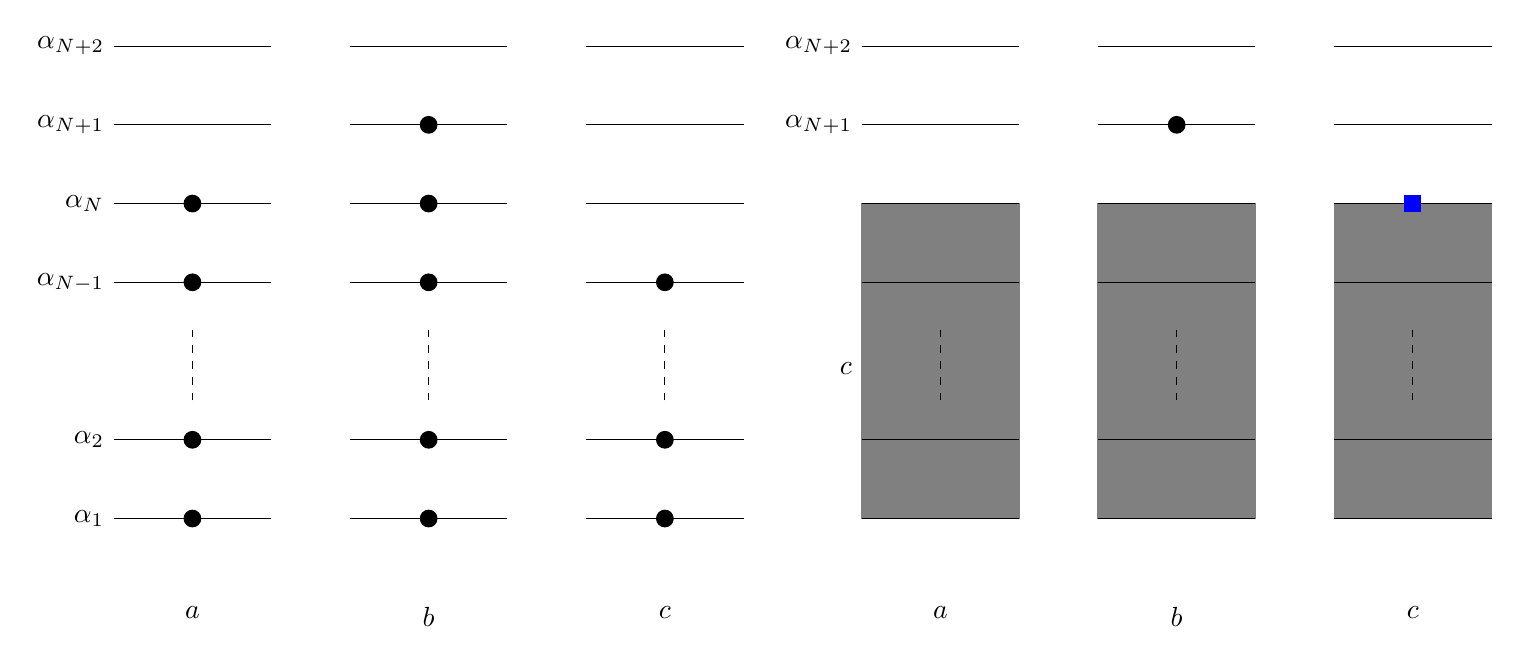
\begin{tikzpicture}
\draw (1,-1) node[anchor=north] {$\ket{a}$} -- (1,-1);
\draw (0,0) node[anchor=east] {$\alpha_1$} -- (2,0);
\draw (0,1) node[anchor=east] {$\alpha_2$} -- (2,1);
\draw (1,1.5) -- (1,1.6);
\draw (1,1.7) -- (1,1.8);
\draw (1,1.9) -- (1,2);
\draw (1,2.1) -- (1,2.2);
\draw (1,2.3) -- (1,2.4);
\draw (0,3) node[anchor=east] {$\alpha_{N-1}$} -- (2,3);
\draw (0,4) node[anchor=east] {$\alpha_N$}-- (2,4);
\draw (0,5) node[anchor=east] {$\alpha_{N+1}$}-- (2,5);
\draw (0,6) node[anchor=east] {$\alpha_{N+2}$} -- (2,6);
\filldraw [black] (1,0) circle (3pt);
\filldraw [black] (1,1) circle (3pt);
\filldraw [black] (1,3) circle (3pt);
\filldraw [black] (1,4) circle (3pt);

\draw (4,-1) node[anchor=north] {$\ket{b}$} -- (4,-1);
\draw (3,0) -- (5,0);
\draw (3,1) -- (5,1);
\draw (4,1.5) -- (4,1.6);
\draw (4,1.7) -- (4,1.8);
\draw (4,1.9) -- (4,2);
\draw (4,2.1) -- (4,2.2);
\draw (4,2.3) -- (4,2.4);
\draw (3,3) -- (5,3);
\draw (3,4) -- (5,4);
\draw (3,5) -- (5,5);
\draw (3,6) -- (5,6);
\filldraw [black] (4,0) circle (3pt);
\filldraw [black] (4,1) circle (3pt);
\filldraw [black] (4,3) circle (3pt);
\filldraw [black] (4,4) circle (3pt);
\filldraw [black] (4,5) circle (3pt);

\draw (7,-1) node[anchor=north] {$\ket{c}$} -- (7,-1);
\draw (6,0) -- (8,0);
\draw (6,1) -- (8,1);
\draw (7,1.5) -- (7,1.6);
\draw (7,1.7) -- (7,1.8);
\draw (7,1.9) -- (7,2);
\draw (7,2.1) -- (7,2.2);
\draw (7,2.3) -- (7,2.4);
\draw (6,3) -- (8,3);
\draw (6,4) -- (8,4);
\draw (6,5) -- (8,5);
\draw (6,6) -- (8,6);
\filldraw [black] (7,0) circle (3pt);
\filldraw [black] (7,1) circle (3pt);
\filldraw [black] (7,3) circle (3pt);

\draw (10.5,-1) node[anchor=north] {$\ket{a}$} -- (10.5,-1);
\filldraw [gray] (9.5,0) rectangle (11.5,4);
\draw (9.5,0) -- (11.5,0);
\draw (9.5,1) -- (11.5,1);
\draw (10.5,1.5) -- (10.5,1.6);
\draw (10.5,1.7) -- (10.5,1.8);
\draw (10.5,1.9) node[anchor=east] {$\ket{c}\hspace{1cm}$} -- (10.5,2);
\draw (10.5,2.1) -- (10.5,2.2);
\draw (10.5,2.3) -- (10.5,2.4);
\draw (9.5,3)  -- (11.5,3);
\draw (9.5,4)  -- (11.5,4);
\draw (9.5,5) node[anchor=east] {$\alpha_{{N+1}}$} -- (11.5,5);
\draw (9.5,6) node[anchor=east] {$\alpha_{N+2}$} -- (11.5,6);

\draw (13.5,-1) node[anchor=north] {$\ket{b}$} -- (13.5,-1);
\filldraw [gray] (12.5,0) rectangle (14.5,4);
\draw (12.5,0) -- (14.5,0);
\draw (12.5,1) -- (14.5,1);
\draw (13.5,1.5) -- (13.5,1.6);
\draw (13.5,1.7) -- (13.5,1.8);
\draw (13.5,1.9) -- (13.5,2);
\draw (13.5,2.1) -- (13.5,2.2);
\draw (13.5,2.3) -- (13.5,2.4);
\draw (12.5,3) -- (14.5,3);
\draw (12.5,4) -- (14.5,4);
\draw (12.5,5) -- (14.5,5);
\draw (12.5,6) -- (14.5,6);
\filldraw [black] (13.5,5) circle (3pt);

\draw (16.5,-1) node[anchor=north] {$\ket{c}$} -- (16.5,-1);
\filldraw [gray] (15.5,0) rectangle (17.5,4);
\draw (15.5,0) -- (17.5,0);
\draw (15.5,1) -- (17.5,1);
\draw (16.5,1.5) -- (16.5,1.6);
\draw (16.5,1.7) -- (16.5,1.8);
\draw (16.5,1.9) -- (16.5,2);
\draw (16.5,2.1) -- (16.5,2.2);
\draw (16.5,2.3) -- (16.5,2.4);
\draw (15.5,3) -- (17.5,3);
\draw (15.5,4) -- (17.5,4);
\draw (15.5,5) -- (17.5,5);
\draw (15.5,6) -- (17.5,6);
\filldraw [blue] (16.4, 3.9) rectangle (16.6,4.1) ;
\end{tikzpicture}}
\end{center}
\label{fig: Particle-hole figure}
\caption{Particle-Hole.}
\end{figure}

In the same way as we can construct a general slater determinant by letting the ordinary creation operators act on the vacuum state, we are now in a position to construct many-quasiparticle states by letting quasi-particle creation operators act on the reference state $\ket{r}$.
\begin{align}
\ket{ijkl..abcd..}_r \equiv \crequasi{i}\crequasi{j}\crequasi{k}\crequasi{l}..\crequasi{a}\crequasi{b}\crequasi{c}\crequasi{d}..\ket{r}.
\end{align}
To achieve the full potential of the particle-hole formalism, one would have to transform all operators to this representation. This is a tedious excersice which we will not include in this report. 

Wick's theorem in Eq. (\ref{def: Wick's theorem}) is valid for products of quasi-particle creation and annihilation operators, provided that the contractions are defined relative to the reference state. The only nonzero contributions are
\begin{align}
\contraction[0.5ex]{}{\anquasi{\alpha}}{}{\crequasi{\beta}} \anquasi{\alpha}\crequasi{\beta} = \for{r}{\anquasi{\alpha}\crequasi{\beta}}{r} = \delta_{\alpha\beta}.
\end{align}



















